\documentclass[a4paper]{article}

\usepackage{INTERSPEECH2021}
\usepackage{makecell}
\usepackage{listings}
\usepackage[T1]{fontenc}
\usepackage{hyperref}
\usepackage{amsmath}
\usepackage{graphicx}
\graphicspath{ {./assets/} }

\usepackage{etoolbox}
\AtBeginEnvironment{quote}{\vspace{-0.5\baselineskip}}% Stuff before {quote}
\AtEndEnvironment{quote}{\vspace{0.05\baselineskip}}% Stuff after {quote}

\title{Final NLU project}
\name{Davide Guidolin (232224)}

\renewcommand\theadalign{bc}
\renewcommand\theadfont{\bfseries}
\renewcommand\theadgape{\Gape[4pt]}
\renewcommand\cellgape{\Gape[4pt]}

\address{
  University of Trento}
\email{davide.guidolin@studenti.unitn.it}

\begin{document}

\maketitle

\begin{abstract}
This is the report for the final project of the course Natural Language Understanding A.Y. 2021/2022. The aim of the project
was to implement a language model using a recurrent neural network architecture and use that model to reach a perplexity lower 
than $90.7$ on the \textit{Penn Treebank} dataset \cite{PTB}.

Along with the report, a Google Colaboratory nootebook with the code is provided. \footnote{\url{https://colab.research.google.com/drive/1YtvMOG_NV_GIgWIFkMrchR5acOQrNuwE?usp=sharing}.}\\
\end{abstract}

\section{Introduction}
The project was started by downloading and analyzing the dataset. Then LSTM has been chosen as RNN architecture and
a simple model was implemented to act as baseline. 

The next step was to follow the suggestions presented in the paper \textit{Regularizing and Optimizing LSTM Language Models} \cite{Merity} 
by \textit{Merity et al.}.

Firstly, the regularization techniques proposed there have been implemented, then some optimization and training algorithms
have been implemented. 

Using both regularization and optimization together, the implemented model have been able to reach a better perplexity than $90.7$.
Finally, some analysis on the best model have been performed.

\section{Task Formalisation}
Language modeling is a subfield of natural language processing (NLP) that focuses on the task of predicting the 
next word in a sequence given the previous words. 
Language models are used in a variety of applications, such as speech recognition, machine translation, and text generation.

A language model is trained on a large dataset of text and learns the statistical properties of the language in the dataset. 
The goal of language modeling is to learn a model $M$ that can predict the probability of a word $w$ at position $t$ in a 
sequence of words $X$, based on the words that come before it:

$$P(w_t | w_1, w_2, ..., w_{t-1}) = M(w_t | w_1, w_2, ..., w_{t-1})$$

Language models can be divided into two categories: statistical language models and neural language models. Both types try to estimate
the distribution of words in the language, however, while statistical models use statistical methods like N-grams or Hidden Markov models,
neural models use neural networks to model the dependencies between words.
Through the years, neural models have shown to be more powerful than statistical models even if they require more data and more
computational power for the training phase.

This project focuses on neural models, specifically LSTM networks have been used for the experiments.

\section{Data Description and Analysis}

\begin{table}
    \begin{center}
        \def\arraystretch{1.2}
        \begin{tabular}{ |c|c|c|c| }
            \hline
            \thead{Split} & \thead{$\#$sentences} & \thead{vocabulary length} & \thead{$\#$words}\\
            \hline\hline
            train & 42068 & 9999 & 887521 \\  
            \hline
            validation & 3370 & 6021 & 70390 \\
            \hline
            test & 3761 & 6048 & 78669 \\
            \hline
        \end{tabular}\\
    \end{center}
    \caption{PTB dataset statistics}
    \label{table:dataset}
\end{table}
\begin{table}
    \begin{center}
        \hspace*{-0.7cm}
        \def\arraystretch{1.2}
        \begin{tabular}{ |c|c|c|c|}
            \hline
            \thead{Split} & \thead{min \\ sentence length} & \thead{max \\ sentence length} & \thead{average \\ sentence length} \\
            \hline\hline
            train & 1 & 82 & 21\\  
            \hline
            validation & 1 & 74 & 21\\
            \hline
            test & 1 & 77 & 21\\
            \hline
        \end{tabular}
    \end{center}
    \caption{PTB sentences lengths}
    \label{table:PTBsentences}
\end{table}
For the training, validation and testing of the models the Penn Treebank (PTB) \cite{PTB} dataset was used. The dataset contains a set 
of annotated stories from a three year Wall Street Journal collection.
The dataset comes already divided in three splits. The training set represents $85.6\%$ of the dataset, the validation set $6.8\%$ 
and the test set $7.6\%$.

In \textit{Table \ref{table:dataset}} the number of sentences, the length of 
the vocabulary and the number of words for each split are reported, while in \textit{Table \ref{table:PTBsentences}} 
the minimum, maximum and average length of the sentences in each split are reported.
Even if the validation and test set are quite small, they contain \textasciitilde{}$60\%$ of the vocabulary words. 
It is important to point out that there are no out-of-vocabulary words in the validation and test set.
From \textit{Table \ref{table:PTBsentences}} it can also be noticed that in the three sets the sentences lengths are balanced.

The dataset has been preprocessed by the authors and all the words were lower-cased, the numbers were replaced with \lstinline{N},
the punctuation was removed and the vocabulary is formed by the most frequent 9999 words, the other tokens were replaced with 
\lstinline{<unk>}.

\begin{table}
    \begin{center}
        \def\arraystretch{1.2}
        \begin{tabular}{ |c|c|c|c| }
            \hline
            \thead{Token} & \thead{Train (\%)} & \thead{Validation (\%)} & \thead{Test (\%)} \\
            \hline\hline
            the & 5.72 & 5.86 & 5.76\\  
            \hline
            <unk> & 5.07 & 4.95 & 6.09\\
            \hline
            N & 3.66 & 3.70 & 3.21\\
            \hline
            of & 2.75 & 2.60 & 2.79\\
            \hline
            to & 2.75 & 2.49 & 2.60\\
            \hline
            a & 2.39 & 2.47 & 2.31\\
            \hline
            in & 2.03 & 1.98 & 2.08\\
            \hline
            and & 1.97 & 1.98 & 1.96\\
            \hline
        \end{tabular}\\
    \end{center}
    \caption{PTB top words frequencies}
    \label{table:frequencies}
\end{table}
In \textit{Table \ref{table:frequencies}} the frequencies of the most frequent tokens in the three splits as percentage over the total 
number of words in the split are reported. Except for \lstinline{<unk>} and \lstinline{N} tokens, all the other tokens are prepositions, 
articles and conjunctions. Except for the \lstinline{<unk>} token, the frequencies across the three splits are very similar.

\section{Model}
Before training the models an \lstinline{<EOS>} token was appended to each sentence to delimit the end of the sentences. 
Then the sentences were tokenized using the \lstinline{split(' ')} Python function and each word was converted to a number in 
an incremental way. During the creation of the dataloaders a \lstinline{<PAD>} token was used to pad each sentence 
to match the length of the longest sentence in the batch and, to create the labels, the ground truth sentences have been shifted left by one word.
The batch size is $32$.

All the experiments were perfomed using a three-layer LSTM network with 400 units in the hidden layers and an embedding size of
400.
For all the experiments $1$ was used as learning rate and $50$ as number of epochs. During training, the gradients were clipped
with a maximum norm of $0.25$. Stochastic gradient descent was used as optimizer.

The first step was to train a baseline model without any regularization technique (SimpleLSTM Model). Then the same model was trained
using early stopping to prevent the overfitting that was occuring after \textasciitilde{}$8$ epochs (SimpleLSTM\_ES Model). 
To implement early stopping a patience variable was used. The patience is decreased if the validation loss is higher than the best loss 
and increased up to a maximum value if the validation loss is lower than the best loss. $5$ was used as starting and maximum patience.

In all the next experiments early stopping will not be used anymore as it has been noticed that with a low patience the model 
stopped too early and there could have been more space for improvement, with a high patience the training stopped too far from 
the minima. $50$ was chosen as number of epochs, because most of the model converged around that epoch, or, if they converged 
before, they didn't overfit much.

The next step was to implement the regularization techniques presented in \cite{Merity}, i.e. various dropout techniques. The first 
technique that was implemented is a simple dropout layer after the embedding and after the lstm output (Dropout Model). 

The second implemented technique was weight dropout (or DropConnect)\cite{DropConnect} that is used to apply dropout on the hidden-to-hidden 
weights of a lstm (WeightDrop Model). Using weight dropout the dropout mask remains the same for the entirety of the forward and backward pass.
Moreover, the dropout operation is applied once on the weights of the network, before the forward and backward pass, 
in this way weight dropout can be applied without any modifications to the LSTM architecture. 

After weight dropout, variational dropout \cite{Variational} was implemented and applied on the embedding and on the lstm output (Variational Model).
In classical dropout new dropout masks are sampled even if the given connection
is repeated, such as the input $x0$ to an LSTM at timestep $t = 0$ receiving a different dropout mask than the input
$x1$ fed to the same LSTM at $t = 1$. With variational dropout the model uses the same dropout mask for all inputs and outputs of 
the LSTM within a given forward and backward pass. 

As last regularization technique embedding dropout was implemented (EmbDropout model). Embedding dropout performs the dropout on the embedding 
matrix using the same mask for a full forward pass, this means that the same words will be dropped during a forward pass.

Finally all the above techniques were used in a single model, however, on the embedding, classical dropout has been used since it 
gave the best results between the three dropout techniques used on the embedding (AllDropout model). So in the final model there will be dropout on the embedding,
weight dropout on the lstm hidden layers and variational dropout on the lstm output.

Then \textit{truncated backpropagation through time (TBPTT)} and \textit{non-monotonically triggered averaged SGD (NT-ASGD)} 
have been implemented.

Truncated backpropagation through time (TBPTT) will perform Backpropagation through time (BPTT) on $k2$ inputs, 
every $k1$ steps. If $k1 = k2$ then it's like splitting the inputs in smaller sequences of $k1$ items and running 
BPTT on the smaller sequences. A value of $k1 = k2$ have been used for all the experiments, however, 
as proposed in \textit{Merity et al.}\cite{Merity} variable length sequences have been used. 
The split size is chosen using a normal distribution $N(25,5)$ with propability $0.95$ and 
$N(12.5, 5)$ with propability $0.05$. 25 was chosen as split average value because the average sentence length is 21 
so most of the time the entire sentence will be selected, some time it will be split.

Non-monotonically triggered averaged SGD (NT-ASGD) is used to switch from SGD to averaged SGD (ASGD) \cite{ASGD}.
ASGD takes the average of the SGD steps in order to reduce the noise and it has been shown to better converge to a minimum, 
so it is triggered when SGD converge to a neighborhood around a solution.
In practice, when the validation perplexity of the model does not decreases in $5$ consecutive steps the optimizer is switched
from SGD to ASGD.

\section{Evaluation}
To measure the performance of a language model the most used metric is perplexity, which is the inverse of 
the probability of the test set, normalized by the number of words. For a test set $W = w_1, w_2, ..., w_N $:
\begin{equation}
    \begin{split}
    PP(W) = \sqrt[N]{\frac{1}{P(w_1,w_2,...,w_N)}} \\
    = \sqrt[N]{\prod_{i=1}^{N}\frac{1}{P(w_i|w_1, ..., w_{i-1})}}
    \end{split}
\end{equation}

Perplexity is a measure of how well the model predicts the test set and a lower perplexity indicates a better model.
The perplexity between two distributions $P$ and $Q$ can also be defined as:
$$ PP(P, Q) =  2^{CE(P, Q)} $$

where $CE()$ is the cross entropy function. This is useful because the model loss will be computed using the cross entropy loss 
so the perplexity of the model can be computed as:

$$ PP(W) = 2^{L(M, W)} $$

where $ L(M, W) $ is the normalized loss of the model on the test set $W$.
The PyTorch cross entropy loss function was used and it already computed the mean of the losses, then the loss was normalized by 
the batch size and the perplexity was computed using this normalized loss. During the loss computation the \lstinline{<PAD>} tokens
have been ignored.

\begin{table}
    \begin{center}
        \def\arraystretch{1.2}
        \begin{tabular}{ |c|c|c| }
            \hline
            \thead{Model} & \thead{Base Model} & \thead{TBPTT + ASGD} \\
            \hline\hline
            SimpleLSTM & 387.56 & - \\  
            \hline
            SimpleLSTM\_ES & 127.77 & - \\
            \hline
            Dropout & \textbf{93.62} & \textbf{93.05} \\
            \hline
            WeightDrop & 121.84 & 109.66 \\
            \hline
            Variational & 98.68 & 95.03 \\
            \hline
            EmbDropout & 173.33 & 166.65 \\
            \hline
        \end{tabular}\\
    \end{center}
    \caption{Perplexities on the test set for the dropout techniques}
    \label{table:test_perplexity_dropout}
\end{table}

\begin{table}
    \begin{center}
        \hspace*{-1cm}
        \def\arraystretch{1.2}
        \begin{tabular}{ |c|c|c|c|c| }
            \hline
            \thead{Model} & \thead{Base Model} & \thead{TBPTT} & \thead{ASGD} & \thead{TBPTT + ASGD} \\
            \hline\hline
            AllDropout & 87.75 & 93.08 & \textbf{83.68} & 88.22 \\  
            \hline
        \end{tabular}\\
    \end{center}
    \caption{Perplexities on the test set for the AllDropout model}
    \label{table:test_perplexity_AllDropout}
\end{table}

In \textit{Table \ref{table:test_perplexity_dropout}} the perplexities of the models on the test set are reported. 
The table has three columns, the second column contains the perplexities of the models trained without TBPTT and ASGD,
the third column contains the perplexities of the same models trained using TBPTT and ASGD. To focus on the best models, the training of SimpleLSTM and SimpleLSTM\_ES
using TBPTT and ASGD was skipped. 
From \textit{Table \ref{table:test_perplexity_dropout}} it can be seen that dropout gives the best results when used alone, while embedding dropout performs even worse
than the SimpleLSTM model. For this reason the use of dropout on the embedding was preferred over embedding dropout on the AllDropout model. Another thing that can be 
noticed from \textit{Table \ref{table:test_perplexity_dropout}} is that TBPTT + ASGD gives a nice boost to the performances of the models, with WeightDrop gaining the 
most advantage. In reality, AllDropout will prove that the advantage is given only by ASGD.

In \textit{Table \ref{table:test_perplexity_AllDropout}} the evaluation of the AllDropout LSTM is reported. This was the best model, and the only one that was able to 
reach a better perplexity than $90.7$. 
First of all it is interesting to see that dropout alone gives the best performances between the other dropout techniques, but it is ouperformed when combined with 
techniques that gave worse results. 
By looking at \textit{Table \ref{table:test_perplexity_AllDropout}} it can be seen that the base model was able to reach a better perplexity than the target perplexity, 
however, by using TBPTT, the perplexity is \textasciitilde{}$5$ points worse. Using ASGD the model gives the best perplexity of $83.68$, while using TBPTT + ASGD the perplexity was 
better than TBPTT alone but still worse than the base model. Different split sizes for TBPTT have been tried but the outcome was the same, so, unless unseen bugs in the code, 
it is evident that TBPTT does not help the model to improve. On the contrary ASGD permits to improve the base model by \textasciitilde{}$4$ points, and this can be clearly seen on 
\textit{Fig. \ref{fig:val_ppl}} that shows the validation perplexity during the training of the four AllDropout models. Around epoch 
$24$ and $27$, i.e. when SGD is replaced by ASGD, the validation perplexity of the models that use ASGD starts to decrease more
to stabilize again a few epochs later.

To better understand the capabilities of the model, an analysis on the frequencies of the generated tokens was performed.
In particular the frequencies of the generated tokens have been compared to the frequencies of the test set tokens. This was
done to see if the frequency distribution of tokens in the model matched the frequency distribution of tokens in the test set. 
In \textit{Table \ref{table:AllDropout_frequency}} this comparison is reported for the best model, i.e. AllDropout with ASGD, the AllDropout model and the test set.
In the table it is also reported the difference between the models frequencies and the ground truth frequencies. In this case the AllDropout Model was chosen for the comparison 
since it gave the lower perplexity between the models without optimization.
Note that the ground truth frequencies reported here are sligthly different from the ones reported in the dataset analysis above,
since to create the labels the sentences have been shifted left by one word, so the first word is missing from the ground truth.

The first thing to notice is the very high frequency of \lstinline{"<unk>"}, \lstinline{"the"} and \lstinline{"<EOS>"} tokens.
\lstinline{"<unk>"} and \lstinline{"the"} are the dominant tokens on the training set while an \lstinline{"<EOS>"} token have been added
to each sentence of the training set, so the model may have overfitted on these tokens due to the high presence in the training set. Regarding the other tokens, the AllDropout ASGD model 
produces the most similar distribution to the ground truth, in particular, the \lstinline{"and"} token appears with almost the same frequency of the 
ground truth, having only $0.01$ percentage points of difference. The AllDropout model produces better frequencies for \lstinline{"<unk>"}, 
\lstinline{"the"} and \lstinline{"to"} tokens, while the frequency distribution of the other tokens is worse than AllDropout ASGD.
The frequencies comparisons for all the other models can be found in the provided nootebook.

\begin{table}[h]
    \begin{center}
        \hspace*{-0.7cm}
        \def\arraystretch{1.2}
        \setlength\tabcolsep{2pt}
        \begin{tabular}{ |c|c|c|c||c|c| }
            \hline
            \thead{Token} & \thead{Test \\set \%} & \thead{AllDropout\\ASGD \%} & \thead{AllDropout\%} & \thead{$\Delta$ \\AllDropout\\ASGD} & \thead{$\Delta$ \\AllDropout}\\
            \hline\hline
            <unk> & 5.85 & 18.32 & 18.77 & 12.47 & 11.76\\  
            \hline
            the & 5.04 & 14.77 & 14.86 & 9.73 & 8.90\\
            \hline
            <EOS> & 4.78 & 10.87 & 10.26 & 6.09 & 6.46\\
            \hline
            a & 2.21 & 2.96 & 3.05 & 0.75 & 1.13\\
            \hline
            of & 2.77 & 4.56 & 4.31 & 1.79 & 1.90\\
            \hline
            to & 2.57 & 3.34 & 3.27 & 0.77 & 0.48\\
            \hline
            and & 1.87 & 1.88 & 1.90 & 0.01 & -0.08\\
            \hline
            N & 3.17 & 3.77 & 3.89 & 0.60 & 0.76\\
            \hline
        \end{tabular}\\
    \end{center}
    \caption{Tokens frequencies comparison between ground truth, AllDropout ASGD and AllDropout}
    \label{table:AllDropout_frequency}
\end{table}

\begin{figure}[h]
    %\centering
    \hspace*{-1.9cm}
    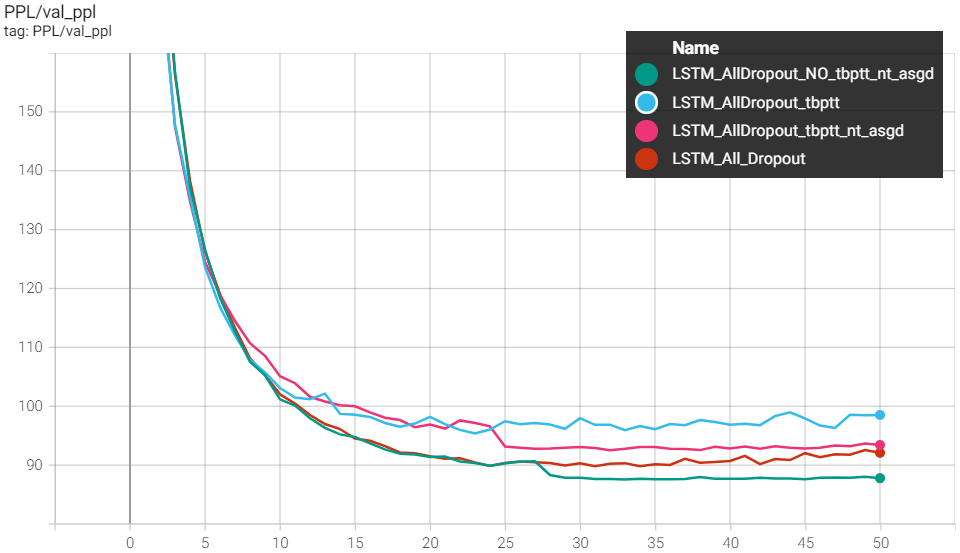
\includegraphics[width=0.63\textwidth]{ValPPL}
    \caption{Validation Perplexities for the four AllDropout models}
    \label{fig:val_ppl}
\end{figure}

To further test the models, some sentences were generated starting from a prompt that could be a word or part of a sentence.
Here some generated sentences are reported, along with the initial prompt. The model used for the generation is AllDropout ASGD.

"the":
\begin{quote}
    the <unk> <unk> <unk> <unk> <unk> <unk> <unk> <EOS>
\end{quote}

"a":
\begin{quote}
    a <unk> <unk> <unk> <unk> <unk> <unk> <EOS>
\end{quote}

"directors":
\begin{quote}
    directors of <unk> <unk> <unk> and <unk> <unk> <EOS>
\end{quote}

"the stock":
\begin{quote}
    the stock market 's plunge was N N <EOS>
\end{quote}

"the company ceo has":
\begin{quote}
    the company ceo has been <unk> <EOS>
\end{quote}

"stock volume is at its":
\begin{quote}
    stock volume is at its <unk> <EOS>
\end{quote}

"the lawyers said":
\begin{quote}
the lawyers said they were n't aware of the allegations <EOS>
\end{quote}

It is clear that the model is too overfitted on \lstinline{"<unk>"} token and the only sentence that has a meaning is the one starting with "The lawyers said". 
To overcome this issue, during the generation, the \lstinline{"<unk>"} token has been replaced with the second most probable word
that the model gave as output.
Here some sentences generated using the just described method are reported.

"the":
\begin{quote}
    the company also has N million common shares <EOS>
\end{quote}

"a":
\begin{quote}
    a spokesman for the parent of the parent of the company said the company is n't interested <EOS>
\end{quote}

"directors":
\begin{quote}
    directors said the plan would allow the president of a holding company to acquire the company 's shares <EOS>
\end{quote}

"the stock":
\begin{quote}
    the stock closed at N cents a pound up \$ at \$ <EOS>
\end{quote}

"the company ceo has":
\begin{quote}
    the company ceo has been able to sell its N N stake in the company <EOS>
\end{quote}

"stock volume is at its":
\begin{quote}
    stock volume is at its level of about \$ N million <EOS>
\end{quote}

"the lawyers said":
\begin{quote}
the lawyers said they were n't aware of any wrongdoing but they did n't have a claim <EOS>
\end{quote}

Now almost all the sentences have a meaning and the model is usable. Moreover, some sentences are really good, like the one starting with "the lawyers said".

\section{Conclusion}
In this project it has been shown how an LSTM network can be greatly improved by using some
simple regularization techniques. Moreover, it has been shown that the optimizer
can dramatically influence the final performance of a neural network. Then, the best model have been 
analyzed and it has been highlighted the overfitting on some very frequent tokens. Finally, the model
have been used to generate some sentences to remark the overfitting on some tokens and a simple solution
has been proposed to overcome this issue and make the model usable.

\bibliographystyle{IEEEtran}

\bibliography{mybib}

\end{document}
